\documentclass[11pt,a4paper]{article}

% ── Packages ──────────────────────────────────────────────────────────
\usepackage[UTF8]{ctex}               % Chinese support
\usepackage{amsmath,amssymb,amsthm}   % Math
\usepackage{mathtools}                % Extended math
\usepackage{bm}                       % Bold math
\usepackage{graphicx}                 % Figures
\usepackage{hyperref}                 % Hyperlinks
\usepackage{cleveref}                 % Smart references
\usepackage{algorithm,algpseudocode}  % Pseudocode
\usepackage{booktabs}                 % Tables
\usepackage[margin=1in]{geometry}     % Page layout
\usepackage{enumitem}                 % Lists
\usepackage{xcolor}                   % Colors
\usepackage{multirow}                 % Multi-row tables
\usepackage{tikz}                     % Diagrams
\usetikzlibrary{arrows.meta,shapes,positioning,fit,backgrounds,calc}

% ── Theorem Environments ───────────────────────────────────────────────
\theoremstyle{plain}
\newtheorem{theorem}{Theorem}[section]
\newtheorem{lemma}[theorem]{Lemma}
\newtheorem{corollary}[theorem]{Corollary}
\newtheorem{proposition}[theorem]{Proposition}

\theoremstyle{definition}
\newtheorem{definition}[theorem]{Definition}
\newtheorem{assumption}[theorem]{Assumption}
\newtheorem{example}[theorem]{Example}

\theoremstyle{remark}
\newtheorem{remark}[theorem]{Remark}

% ── Custom Commands ────────────────────────────────────────────────────
\newcommand{\SCX}{\text{SCX}}
\newcommand{\Cercis}{\text{Cercis}}
\newcommand{\Situs}{\text{Situs}}
\newcommand{\bbR}{\mathbb{R}}
\newcommand{\bbN}{\mathbb{N}}
\newcommand{\bbE}{\mathbb{E}}
\newcommand{\bbP}{\mathbb{P}}
\newcommand{\bbV}{\mathbb{V}}
\newcommand{\cA}{\mathcal{A}}
\newcommand{\cB}{\mathcal{B}}
\newcommand{\cD}{\mathcal{D}}
\newcommand{\cE}{\mathcal{E}}
\newcommand{\cF}{\mathcal{F}}
\newcommand{\cG}{\mathcal{G}}
\newcommand{\cH}{\mathcal{H}}
\newcommand{\cN}{\mathcal{N}}
\newcommand{\cO}{\mathcal{O}}
\newcommand{\cS}{\mathcal{S}}
\newcommand{\cX}{\mathcal{X}}
\newcommand{\cY}{\mathcal{Y}}
\newcommand{\indep}{\perp\!\!\!\perp}
\newcommand{\norm}[1]{\left\lVert#1\right\rVert}
\newcommand{\abs}[1]{\left\lvert#1\right\rvert}
\newcommand{\inprod}[2]{\langle #1, #2 \rangle}
\newcommand{\indicator}{\mathbf{1}}
\newcommand{\TODO}[1]{\textcolor{red}{[TODO: #1]}}

% ── Title ──────────────────────────────────────────────────────────────
\title{
  \textbf{The Goodhart Gauge: Formal Detection and Mitigation of\\
  Metric Manipulation in the Cercis Score Framework}\\[0.5\baselineskip]
  \large 古德哈特度量：Cercis评分框架下度量操纵的形式化检测与缓解
}

\author{
  SCX Research Collective\\
  \texttt{hermes-agent@nousresearch.com}
}

\date{July 2026}

\begin{document}
\maketitle

% ═══════════════════════════════════════════════════════════════════════
\begin{abstract}
\noindent
\textbf{English.}
Goodhart's Law states that ``when a measure becomes a target, it ceases to be a good measure.''
In the SCX egalitarian framework, the Cercis Score $S(x) = Q(x) + \eta N(x)$ aggregates
quality $Q$ and novelty $N$ into a single scalar objective. Should this score become an
optimization target for self-interested agents---data providers, expert auditors, or
state-level actors---the framework is vulnerable to metric manipulation that decouples
$S$ from its underlying semantics. This paper formalizes three distinct attack surfaces:
(i) \emph{data inflation}, where agents artificially inflate quality metrics without
improving genuine quality; (ii) \emph{expert collusion}, where multiple auditors coordinate
to fabricate consensus; and (iii) \emph{state forgery}, where adversaries synthesize entire
evaluation states to masquerade as authentic Cercis landscapes. For each threat, we prove
detection bounds that establish the minimum sample complexity required to distinguish
manipulated scores from legitimate ones with high probability. We then propose a layered
defense architecture comprising independent audit rotation, state-coverage penalties, and
multi-expert independence testing, each accompanied by formal guarantees.
\\[0.3\baselineskip]
\noindent
\textbf{中文.}
古德哈特定律指出：「当一项度量成为目标时，它就不再是好的度量。」在SCX平等论框架中，
Cercis分数 $S(x)=Q(x)+\eta N(x)$ 将质量 $Q$ 与新颖性 $N$ 聚合为单一标量目标。
一旦该分数成为自利主体——数据提供者、专家审计员或国家级行为者——的优化目标，
框架将面临度量操纵的风险，使得 $S$ 与其底层语义脱钩。本文形式化三种攻击面：
（一）\textbf{数据膨胀}，即主体人为抬高质量度量而不改善真实质量；
（二）\textbf{专家共谋}，即多名审计员协调伪造共识；
（三）\textbf{状态伪造}，即对手合成完整评估状态以伪装为真实的Cercis景观。
针对每种威胁，我们证明检测边界，建立以高概率区分操纵分数与合法分数所需的最小样本复杂度。
随后提出分层防御架构，包括独立审计轮换、状态覆盖度惩罚与多专家独立性检验，每项附有形式化保证。
\end{abstract}

% ═══════════════════════════════════════════════════════════════════════
\section{Introduction}
\label{sec:intro}

\subsection{Motivation}

Goodhart's Law, named after the economist Charles Goodhart who observed that
``any observed statistical regularity will tend to collapse once pressure is
placed upon it for control purposes''~\cite{goodhart1975problems}, has become a
central concern in the age of AI evaluation. When a scalar metric---be it
test-set accuracy, BLEU score, or human-preference rating---becomes the
objective that systems or humans optimize against, the metric's correlation
with the underlying construct it was designed to measure degrades, often
catastrophically.

\smallskip
\noindent
\textbf{古德哈特定律的现代诠释.} 在AI评估领域，Goodhart警告转化为一个精确的技术问题：
是否存在一种度量体系，其被操纵的难度（操纵成本）在数学上可界定，且其被操纵的事实
（操纵检测）在统计上可证明？SCX平等论框架试图通过Cercis Score $S$ 回答这一问题，
但框架本身尚未形式化其面对Goodhart攻击时的鲁棒性边界。

The SCX egalitarian framework~\cite{scx2025} defines the Cercis Score as:
\begin{equation}\label{eq:cercis_def}
  S(x) = Q(x) + \eta \cdot N(x),
\end{equation}
where $Q(x)$ is the intrinsic quality of artifact $x$, $N(x)$ is its novelty
relative to the existing corpus, and $\eta > 0$ is the novelty-weighting
parameter. The score lives on the Situs manifold $(\mathcal{X}, d_P, \mu_P)$,
where $d_P$ encodes perceptual distance and $\mu_P$ encodes the empirical
distribution of artifacts.

\medskip
\noindent
\textbf{The Goodhart Threat.} Consider an adversary who can observe (or
estimate) the Cercis Score $S(x)$ and wishes to maximize it without incurring
the cost of genuine quality improvement. Three canonical attack strategies
emerge:

\begin{enumerate}[label=\textbf{A\arabic*}, leftmargin=*]
  \item \textbf{Data Inflation (A1).} The adversary generates artifacts $\tilde{x}$
        that score highly on $S$ by exploiting blind spots in the $Q$ estimator,
        without improving true quality. This is the analog of ``teaching to the test.''
  \item \textbf{Expert Collusion (A2).} Multiple auditors $\{E_k\}_{k=1}^K$ collude
        to report inflated or coordinated scores that mimic genuine inter-rater
        disagreement patterns while systematically shifting the consensus upward.
  \item \textbf{State Forgery (A3).} The adversary synthesizes an entire evaluation
        state---a tuple $(x, S(x), \nabla S(x), H_S(x))$---that is indistinguishable
        from authentic Cercis states to the downstream consumer (model trainer,
        policy maker, funding agency).
\end{enumerate}

\subsection{Contributions}

This paper makes the following contributions:

\begin{enumerate}[label=\textbf{C\arabic*}, leftmargin=*]
  \item \textbf{Threat Formalization} (Section~\ref{sec:threat}). We provide rigorous
        mathematical definitions of A1--A3 within the SCX framework, specifying the
        adversary's capabilities, knowledge, and objective for each attack surface.

  \item \textbf{Detection Bounds} (Section~\ref{sec:bounds}). For each attack, we prove
        a detection theorem that quantifies the minimum number of samples $n$ required to
        reject the null hypothesis of ``no manipulation'' at significance level $\alpha$
        with power $1-\beta$. The bounds expose an inherent detection-manipulation
        trade-off governed by the Cercis novelty parameter $\eta$.

  \item \textbf{Countermeasure Architecture} (Section~\ref{sec:defense}). We propose
        three defense mechanisms with formal guarantees:
        (a) independent audit rotation, which decorrelates auditor assignments to break
        collusion equilibria; (b) state-coverage penalties, which penalize concentration
        of evaluated artifacts in regions of Situs space; and (c) multi-expert
        independence testing, which detects collusion via conditional independence
        violations.

  \item \textbf{Bilingual Exposition} (throughout). All theorems, definitions, and
        interpretations are presented in both English and Chinese to serve the
        international SCX research community. 全文以中英双语呈现，服务国际SCX研究共同体。
\end{enumerate}

\subsection{Related Work}

Goodhart's law has been studied extensively in economics~\cite{goodhart1975problems,strathern1997improving},
machine learning~\cite{manheim2019categorizing,karwowski2024goodhart}, and AI safety~\cite{zhuang2023goodhart,krakovna2020specification}.
Our work differs in three respects: (1) we operate within the specific mathematical
structure of the SCX framework rather than treating evaluation as a black box;
(2) we prove \emph{detection bounds} with explicit dependence on the Cercis parameter
$\eta$, rather than providing qualitative taxonomies; and (3) our countermeasures
are designed to compose with existing SCX theorems (notably Theorem~3 on
noise-difficulty indistinguishability and Theorem~7 on cross-domain preservation).

% ═══════════════════════════════════════════════════════════════════════
\section{Preliminaries: The SCX Framework}
\label{sec:prelim}

\subsection{Cercis Score and Situs Manifold}

We recall the core objects of the SCX framework. Let $\cX$ be the space of all
artifacts (texts, models, datasets, policies). The \textbf{Situs operator}
encodes $\cX$ as a metric measure space:
\begin{equation}\label{eq:situs}
  \Situs: \cX \to (\cX, d_P, \mu_P),
\end{equation}
where $d_P(x,y)$ is a perceptual distance (Wasserstein distance between the
internal representations of $x$ and $y$ under a reference model $P$) and
$\mu_P$ is the empirical distribution of artifacts.

\begin{definition}[Cercis Score]
  \label{def:cercis}
  For any artifact $x \in \cX$, the \textbf{Cercis Score} $S: \cX \to \bbR^+$ is:
  \[
    S(x) = Q(x) + \eta \cdot N(x),
  \]
  where:
  \begin{itemize}
    \item $Q(x) \in [0,1]$ is the intrinsic quality score (expected utility to a
          downstream consumer);
    \item $N(x) = D_{\text{KL}}(\delta_x \| \mu_P)$ or equivalently the Situs-distance
          to the nearest $k$ neighbors, measuring novelty relative to the corpus;
    \item $\eta > 0$ is the novelty-weighting hyperparameter.
  \end{itemize}
\end{definition}

\begin{definition}[Cercis State]
  \label{def:state}
  The \textbf{Cercis state} of artifact $x$ is the tuple:
  \[
    \Sigma(x) = \bigl(x,\; S(x),\; \nabla S(x),\; H_S(x)\bigr),
  \]
  where $\nabla S(x)$ is the gradient of $S$ on the Situs manifold and $H_S(x)$ is
  the Hessian (second-order derivative information). The auditor's observable is
  $\Sigma(x)$; the true quality $Q(x)$ is latent.
\end{definition}

\subsection{Assumptions}

We maintain the standard SCX assumptions~\cite{scx2025}:

\begin{assumption}[A1: Bounded Scores]
  \label{ass:bounded}
  $0 \leq Q(x) \leq 1$ and $0 \leq N(x) \leq N_{\max}$ for all $x \in \cX$.
  Consequently $S(x) \in [0, 1 + \eta N_{\max}]$.
\end{assumption}

\begin{assumption}[A2: Lipschitz Quality]
  \label{ass:lipschitz}
  $Q$ is $L_Q$-Lipschitz on the Situs manifold: $|Q(x) - Q(y)| \leq L_Q \cdot d_P(x,y)$.
\end{assumption}

\begin{assumption}[A3: Independent Audit Noise]
  \label{ass:audit_noise}
  Expert $k$ observes $S_k(x) = S(x) + \varepsilon_k$, where $\varepsilon_k \sim \cN(0,\sigma_k^2)$
  independently across experts and artifacts, with $\sigma_k \leq \sigma_{\max}$.
\end{assumption}

\begin{assumption}[A4: Situs Regularity]
  \label{ass:situs_reg}
  The Situs manifold $(\cX, d_P)$ is compact with diameter $D_{\max} < \infty$,
  and the gradient $\nabla S$ exists almost everywhere with $\|\nabla S(x)\| \leq G_{\max}$.
\end{assumption}

% ═══════════════════════════════════════════════════════════════════════
\section{Threat Model}
\label{sec:threat}

\noindent
\textbf{威胁模型总览.} 我们考虑三类对手，按能力递增排列。所有对手共享目标：
在最小化真实质量改进成本的前提下，最大化其管辖制品的Cercis分数。

\begin{center}
\begin{tabular}{@{}lcccc@{}}
\toprule
\textbf{攻击} & \textbf{对手能力} & \textbf{目标} & \textbf{观测} & \textbf{成本} \\
\midrule
A1: 数据膨胀   & 制品生成     & $\max S(\tilde{x})$     & $Q$的代理估计   & 生成成本 \\
A2: 专家共谋   & 审计协调     & $\max \bar{S}_{\text{rep}}$ & 其他专家的报告 & 协调成本 \\
A3: 状态伪造   & 完全知识     & $\max S(x)$ 无检测      & 完整$\Sigma(x)$  & 伪造成本 \\
\bottomrule
\end{tabular}
\end{center}

% ───────────────────────────────────────────────────────────────────────
\subsection{A1: Data Inflation \quad 数据膨胀}

\begin{definition}[Data Inflation Attack]
  \label{def:a1}
  An adversary $\cA_1$ with access to a surrogate quality estimator $\hat{Q}(\cdot)$
  (which may be a proxy model, a leaked evaluation rubric, or gradient queries to
  the scoring system) produces artifacts $\{\tilde{x}_i\}_{i=1}^m$ satisfying:
  \[
    \hat{S}(\tilde{x}_i) = \hat{Q}(\tilde{x}_i) + \eta \hat{N}(\tilde{x}_i) \geq \tau,
  \]
  for some threshold $\tau$, while
  \[
    \bbE[Q(\tilde{x}_i)] \leq \bbE[\hat{Q}(\tilde{x}_i)] - \Delta_Q,
  \]
  where $\Delta_Q > 0$ is the \textbf{quality gap} between estimated and true quality.
\end{definition}

\noindent
\textbf{核心机制.} 对手利用 $Q$ 与 $\hat{Q}$ 之间的分布偏移生成在代理估计器上得分高
但在真实质量上得分低的制品。这类似乎「应试教育」：学生学会考试技巧（优化 $\hat{Q}$）
而非掌握学科内容（提升 $Q$）。

The quality gap $\Delta_Q$ is the adversary's ``Goodhart margin''---the extent to which
the proxy metric $\hat{Q}$ overestimates true quality $Q$. This gap arises from:

\begin{enumerate}[label=(\roman*)]
  \item \textbf{Estimator incompleteness}: $\hat{Q}$ captures only a subset of the
        quality dimensions that $Q$ measures.
  \item \textbf{Distribution shift}: $\hat{Q}$ was calibrated on a training distribution
        $\cD_{\text{train}}$ that differs from the adversary's generation distribution
        $\cD_{\text{adv}}$.
  \item \textbf{Adversarial overfitting}: the adversary actively searches for inputs
        where $|\hat{Q}(x) - Q(x)|$ is large.
\end{enumerate}

% ───────────────────────────────────────────────────────────────────────
\subsection{A2: Expert Collusion \quad 专家共谋}

\begin{definition}[Expert Collusion Attack]
  \label{def:a2}
  Let $\cE = \{E_1, \dots, E_K\}$ be $K$ expert auditors assigned to evaluate artifact
  $x$. In a collusion attack, a subset $\cE_C \subseteq \cE$ of size $K_C \leq K$
  coordinates to report:
  \[
    S_k^{\text{rep}}(x) = S(x) + \delta + \tilde{\varepsilon}_k,
  \]
  where $\delta > 0$ is a \textbf{collusive bias} (common across colluders) and
  $\tilde{\varepsilon}_k \sim \cN(0, \tilde{\sigma}_k^2)$ are fabricated noise terms
  calibrated to match the variance of honest auditors, i.e., $\tilde{\sigma}_k \approx \sigma_k$.
\end{definition}

\noindent
\textbf{共谋结构.} 共谋者面临一个微妙的设计问题：他们的报告必须同时满足两个条件：
(1) 系统性地偏移均值（$\delta > 0$）以提升聚合分数；
(2) 保持报告之间的表面独立性（$\tilde{\varepsilon}_k$ 匹配 $\sigma_k$）以逃避统计检测。

The colluders' dilemma is that $\delta$ cannot be made arbitrarily large without
being detected by outlier tests, but must be large enough to meaningfully shift the
aggregate score $\bar{S} = \frac{1}{K}\sum_k S_k^{\text{rep}}$.

% ───────────────────────────────────────────────────────────────────────
\subsection{A3: State Forgery \quad 状态伪造}

\begin{definition}[State Forgery Attack]
  \label{def:a3}
  An adversary $\cA_3$ with complete knowledge of the SCX framework (including the
  Situs manifold structure, the Cercis Score definition, and the distribution of
  legitimate evaluation states) produces forged states $\tilde{\Sigma}(x) =
  (\tilde{x}, \tilde{S}, \tilde{\nabla}S, \tilde{H}_S)$ such that the distribution
  $\cD_{\text{forge}}$ of forged states is $\varepsilon$-close to the distribution
  $\cD_{\text{legit}}$ of legitimate states in total variation:
  \[
    d_{\text{TV}}(\cD_{\text{forge}}, \cD_{\text{legit}}) \leq \varepsilon.
  \]
\end{definition}

\noindent
\textbf{状态伪造的严重性.} A3是最强大的攻击：对手不仅操纵分数，而且构造整个评估状态，
包括梯度与Hessian信息，使得审计者无法从可观测量的联合分布中区分真伪。
这与SCX Theorem~3（噪声-难度不可区分性）形成对偶：Theorem 3断言噪声与内在难度
在观测层面不可区分；A3断言在分数与梯度层面也可以构造不可区分的伪造状态。
两者的交集定义了检测可能性的根本边界。

% ═══════════════════════════════════════════════════════════════════════
\section{Detection Bounds}
\label{sec:bounds}

\noindent
\textbf{检测边界总览.} 对每种攻击，我们证明一个检测定理，形式为：
在显著性水平 $\alpha$ 下，以功效 $1-\beta$ 检测操纵所需的最小样本量 $n^*$ 由攻击强度参数
（$\Delta_Q$、$\delta$ 或 $\varepsilon$）以及Cercis新颖性参数 $\eta$ 决定。

% ───────────────────────────────────────────────────────────────────────
\subsection{Detecting Data Inflation}
\label{sec:bound_a1}

\begin{theorem}[Data Inflation Detection Bound]
  \label{thm:a1_detect}
  Let $\cD_{\text{legit}}$ be the distribution of Cercis Scores for authentic artifacts
  with mean $\mu_S$ and variance $\sigma_S^2$. Let $\cD_{\text{infl}}$ be the distribution
  of inflated artifacts with mean $\mu_S + \Delta_{\text{infl}}$ and variance
  $\sigma_S^2 + \Delta_\sigma^2$. Assume $\Delta_Q = \Delta_{\text{infl}} - \eta \cdot \Delta_N$,
  where $\Delta_N \geq 0$ is the novelty shift. Then:

  \begin{enumerate}[label=(\roman*)]
    \item \textbf{Score-based detection.} A two-sample $t$-test on $n$ observed scores
          detects inflation at level $\alpha$ with power $1-\beta$ when:
          \begin{equation}\label{eq:detect_a1}
            n \geq n_{\text{A1}}^* =
            \frac{2(\sigma_S^2 + \Delta_\sigma^2/2)}{\Delta_{\text{infl}}^2}
            \cdot (z_{1-\alpha/2} + z_{1-\beta})^2.
          \end{equation}

    \item \textbf{Gradient-based detection.} If the adversary's artifacts exhibit
          anomalous gradient structure $\|\nabla S(\tilde{x})\| \leq G_{\text{legit}} - \Delta_G$
          (less ``rugged'' than legitimate high-quality artifacts), then detection
          is possible with:
          \begin{equation}\label{eq:detect_a1_grad}
            n \geq n_{\text{A1,grad}}^* =
            \frac{2\sigma_G^2}{\Delta_G^2} \cdot (z_{1-\alpha/2} + z_{1-\beta})^2,
          \end{equation}
          where $\sigma_G^2 = \bbV[\|\nabla S(x)\|]$ under the legitimate distribution.
  \end{enumerate}
\end{theorem}

\begin{proof}
  \textbf{Part (i).} Under the null $H_0$ (no inflation), scores are i.i.d.\ with
  mean $\mu_S$. Under $H_1$ (inflation), scores have mean $\mu_S + \Delta_{\text{infl}}$.
  Let $\bar{S}_n = \frac{1}{n}\sum_{i=1}^n S(x_i)$. By the Central Limit Theorem,
  \[
    \frac{\bar{S}_n - \mu_S}{\sigma_S/\sqrt{n}} \xrightarrow{d} \cN(0,1) \quad \text{under } H_0,
  \]
  and
  \[
    \frac{\bar{S}_n - (\mu_S + \Delta_{\text{infl}})}{\sqrt{(\sigma_S^2 + \Delta_\sigma^2)/n}}
    \xrightarrow{d} \cN(0,1) \quad \text{under } H_1.
  \]
  The standard sample-size formula for a two-sided $z$-test with pooled variance
  $\sigma_{\text{pool}}^2 = \sigma_S^2 + \Delta_\sigma^2/2$ yields~\eqref{eq:detect_a1}.

  \textbf{Part (ii).} Same logic applied to the gradient norm statistic
  $G(x) = \|\nabla S(x)\|$, which under Assumption~\ref{ass:situs_reg} is bounded.
  The separation $\Delta_G$ captures the fact that inflated artifacts, being
  generated to maximize a proxy score, tend to lie in ``flat'' regions of $S$
  (local optima of the proxy) rather than the ``rugged'' regions characteristic
  of genuinely novel, high-quality artifacts. \hfill $\square$
\end{proof}

\begin{remark}[Interpretation]
  \textbf{中文解读.} 检测边界 $n_{\text{A1}}^*$ 揭示了三个关键关系：
  \begin{itemize}
    \item $\Delta_{\text{infl}}$ 越大（质量膨胀越严重），检测所需样本越少
          —— 大尺度的操纵反而更容易被检测到。
    \item $\Delta_\sigma^2$（膨胀伪影引入的额外方差）增加检测难度
          —— 对手可以通过增加噪声来隐藏膨胀信号。
    \item $\eta$ 通过 $\Delta_{\text{infl}} = \Delta_Q + \eta \Delta_N$ 间接影响边界：
          当对手同时操纵新颖性时（$\Delta_N > 0$），更大的 $\eta$ 使膨胀信号更强，
          从而更容易检测。\textbf{这形成一个内在的检测-操纵权衡：$\eta$越大，Cercis分数
          对新事物的奖励越大，但操纵信号的放大也越明显。}
  \end{itemize}

  The trade-off $\eta \uparrow \implies$ (more reward for novelty, easier to detect inflation)
  is a \textbf{self-limiting property} of the Cercis Score: the same mechanism that makes
  the score valuable also makes its manipulation detectable.
\end{remark}

% ───────────────────────────────────────────────────────────────────────
\subsection{Detecting Expert Collusion}
\label{sec:bound_a2}

\begin{theorem}[Expert Collusion Detection Bound]
  \label{thm:a2_detect}
  Let $K$ experts evaluate artifact $x$, of whom $K_C \leq \lfloor K/2 \rfloor$ are
  colluding with common bias $\delta$ and calibrated variance $\sigma_C^2 = \sigma_H^2$,
  where $\sigma_H^2$ is the honest-expert variance. Define the \textbf{inter-expert
  correlation anomaly}:
  \[
    \rho_{\text{anom}} = \frac{\delta^2}{\delta^2 + 2\sigma_H^2}.
  \]
  Then:

  \begin{enumerate}[label=(\roman*)]
    \item \textbf{Pairwise correlation test.} For any pair of colluding experts $(i,j)$,
          the pairwise correlation $\rho_{ij}$ exceeds the null expectation
          $\rho_0 = 0$ (under honesty + independence). A $z$-test on Fisher-transformed
          correlations detects collusion at level $\alpha$ when:
          \begin{equation}\label{eq:detect_a2_corr}
            n \geq n_{\text{A2,corr}}^* =
            \frac{(z_{1-\alpha/2} + z_{1-\beta})^2}
                 {\left(\frac{1}{2}\ln\frac{1+\rho_{\text{anom}}}{1-\rho_{\text{anom}}}\right)^2} + 3.
          \end{equation}

    \item \textbf{Variance ratio test.} The within-group variance of colluding experts
          is systematically lower than the between-group variance. Define the
          \textbf{collusion F-statistic}:
          \begin{equation}\label{eq:collusion_F}
            F_{\text{coll}} = \frac{\text{MS}_{\text{between}}}{\text{MS}_{\text{within}}}
            = \frac{K_C(K - K_C)\delta^2 + \sigma_H^2}{\sigma_H^2}.
          \end{equation}
          Under $H_0$ (no collusion), $F_{\text{coll}} \sim F_{1, K-2}$.
          Detection at level $\alpha$ requires:
          \begin{equation}\label{eq:detect_a2_F}
            n \geq \frac{(\sigma_H^2 / \delta^2) \cdot (F_{1,K-2;1-\beta} - 1)}{K_C(K - K_C)}.
          \end{equation}
  \end{enumerate}
\end{theorem}

\begin{proof}
  \textbf{Part (i): Correlation anomaly.} For two colluding experts $i,j \in \cE_C$,
  their reported scores are:
  \[
    S_i = S + \delta + \varepsilon_i, \quad S_j = S + \delta + \varepsilon_j,
  \]
  where $\varepsilon_i, \varepsilon_j \sim_{\text{i.i.d.}} \cN(0, \sigma_H^2)$.
  The covariance is $\text{Cov}(S_i, S_j) = \bbV[S] + \delta^2$ (common $S$ and common
  $\delta$), while each variance is $\bbV[S_i] = \bbV[S] + \sigma_H^2 + \delta^2$.
  Hence:
  \[
    \rho_{ij} = \frac{\bbV[S] + \delta^2}{\bbV[S] + \sigma_H^2 + \delta^2}.
  \]
  For $\bbV[S] \gg \delta^2$ (natural score variation dominates collusive bias),
  this simplifies to $\rho_{\text{anom}} \approx \delta^2/(\delta^2 + \sigma_H^2)$.
  The Fisher $z$-transformation $z(\rho) = \frac{1}{2}\ln\frac{1+\rho}{1-\rho}$ is
  approximately $\cN(z(\rho), 1/(n-3))$. The sample size formula follows from the
  standard power calculation for the difference $z(\rho_{\text{anom}}) - z(0)$.

  \textbf{Part (ii): ANOVA decomposition.} Consider the one-way ANOVA with groups:
  colluders vs.\ non-colluders. The between-group sum of squares captures the
  systematic bias $\delta$:
  \[
    \text{SS}_{\text{between}} = K_C(\bar{S}_C - \bar{S})^2 + (K-K_C)(\bar{S}_H - \bar{S})^2
    = \frac{K_C(K-K_C)}{K} \delta^2,
  \]
  where $\bar{S}_C = S + \delta$ (colluder mean) and $\bar{S}_H = S$ (honest mean).
  The within-group MS estimates $\sigma_H^2$. Substituting into the $F$-ratio yields
  \eqref{eq:collusion_F}. The noncentrality parameter of the $F$-distribution under
  $H_1$ is $\lambda = n \cdot K_C(K-K_C) \cdot \delta^2 / \sigma_H^2$, from which
  the sample size formula~\eqref{eq:detect_a2_F} follows via the standard noncentral
  $F$ power calculation. \hfill $\square$
\end{proof}

\begin{remark}[Collusion Detectability Phase Transition]
  \textbf{共谋可检测性的相变.} 定义共谋信噪比 $\text{SNR}_C = \delta / \sigma_H$。
  存在临界值：
  \[
    \delta_{\text{crit}} = \sigma_H \cdot \sqrt{\frac{2\ln(1/\alpha)}{K_C(K-K_C)}}.
  \]
  当 $\delta < \delta_{\text{crit}}$ 时，共谋在统计上不可检测（功效 $< 1-\beta$ 对任何有限 $n$）；
  当 $\delta > \delta_{\text{crit}}$ 时，所需样本量随 $1/\delta^2$ 衰减。
  
  这定义了 \textbf{Cercis-Goodhart 相变}：存在一个对手机制不可能同时
  实现（i）显著分数提升（$\delta$ 大）和（ii）统计不可检测性（$\delta < \delta_{\text{crit}}$）
  的参数区域。\textbf{系统设计者可以通过调节 $K$ 和 $\sigma_H$ 来推移 $\delta_{\text{crit}}$，
  使得任何具有实际意义的分数操纵必然落入可检测区域。}
\end{remark}

% ───────────────────────────────────────────────────────────────────────
\subsection{Detecting State Forgery}
\label{sec:bound_a3}

\begin{theorem}[State Forgery Detection Bound]
  \label{thm:a3_detect}
  Let $\cD_{\text{legit}}$ be the joint distribution of Cercis states
  $\Sigma(x) = (x, S, \nabla S, H_S)$ for legitimate artifacts, and let
  $\cD_{\text{forge}}$ be the distribution of forged states.
  Assume that authentic Cercis states satisfy the \textbf{gradient consistency
  condition}:
  \begin{equation}\label{eq:grad_consistency}
    \bbE[\|\nabla S(x) - \nabla_{\Situs} \hat{S}(x)\|^2] \leq \kappa^2,
  \end{equation}
  where $\nabla_{\Situs}$ is the Situs manifold gradient operator and
  $\hat{S}$ is any estimator of $S$. Then:

  \begin{enumerate}[label=(\roman*)]
    \item \textbf{Gradient inconsistency detection.} Define the
          \textbf{curl inconsistency statistic}:
          \begin{equation}\label{eq:curl_stat}
            \tau(x) = \|\nabla \times \nabla S(x)\|^2,
          \end{equation}
          where $\nabla \times$ is the exterior derivative on the Situs manifold.
          For authentic states, $\bbE[\tau(x)] \leq \kappa^2$, while for forged
          states lacking Situs consistency, $\bbE_{\text{forge}}[\tau(x)] \geq \kappa^2 + \Delta_\tau$.
          A one-sided $z$-test on $\bar{\tau}_n$ detects forgery when:
          \begin{equation}\label{eq:detect_a3_curl}
            n \geq n_{\text{A3}}^* =
            \frac{\sigma_\tau^2}{\Delta_\tau^2} \cdot (z_{1-\alpha} + z_{1-\beta})^2,
          \end{equation}
          where $\sigma_\tau^2 = \bbV_{\text{legit}}[\tau(x)]$.

    \item \textbf{Situs geodesic test.} For any pair of forged states
          $(\tilde{\Sigma}_i, \tilde{\Sigma}_j)$, the Situs geodesic distance
          $d_P(\tilde{x}_i, \tilde{x}_j)$ and the score difference
          $|\tilde{S}_i - \tilde{S}_j|$ must satisfy the \textbf{Cercis-Lipschitz
          constraint}:
          \begin{equation}\label{eq:cercis_lipschitz}
            |\tilde{S}_i - \tilde{S}_j| \leq (L_Q + \eta L_N) \cdot d_P(\tilde{x}_i, \tilde{x}_j).
          \end{equation}
          Violations of~\eqref{eq:cercis_lipschitz} constitute detectable anomalies.
          The probability of a random pair violating the constraint under $H_0$ is
          bounded by:
          \[
            \bbP_{H_0}(\text{violation}) \leq
            2\exp\left(-\frac{(L_Q + \eta L_N)^2 \cdot d_{\min}^2}{2\sigma_S^2}\right),
          \]
          where $d_{\min} = \min_{i \neq j} d_P(\tilde{x}_i, \tilde{x}_j)$.
  \end{enumerate}
\end{theorem}

\begin{proof}
  \textbf{Part (i):} The key insight is that on a smooth manifold with a metric
  connection (Levi-Civita), the curl of a gradient field is identically zero:
  $\nabla \times \nabla f \equiv 0$ for any smooth $f$. Forged states generated
  without solving the Situs consistency constraints will typically violate this
  identity, producing a non-zero curl statistic. Under $H_0$, $\tau(x) \approx 0$
  (up to discretization error $\kappa$); under $H_1$, $\tau(x)$ is inflated by
  $\Delta_\tau$. The sample size formula follows from the standard power calculation
  for a one-sided $z$-test.

  \textbf{Part (ii):} The Cercis-Lipschitz constraint follows from Assumptions~\ref{ass:lipschitz}
  and~\ref{ass:situs_reg}:
  \[
    |S(x) - S(y)| = |(Q(x) - Q(y)) + \eta(N(x) - N(y))|
    \leq L_Q d_P(x,y) + \eta L_N d_P(x,y).
  \]
  Under $H_0$, score differences between random pairs are approximately normal with
  variance $2\sigma_S^2$. The tail bound follows from Hoeffding's inequality applied
  to the event $\{|S_i - S_j| > (L_Q + \eta L_N) d_P(x_i, x_j)\}$. \hfill $\square$
\end{proof}

\begin{remark}[The Fundamental Tension with Theorem 3]
  \textbf{与Theorem 3的基础张力.} SCX Theorem~3 断言：从观测数据 $(S, \nabla S, H_S)$
  无法区分标签噪声与内在难度。状态伪造检测（A3检测）似乎与这一断言矛盾
  —— 如果噪声与难度不可区分，那么伪造状态（模拟噪声结构）也应不可区分。

  消解这一表面矛盾的关键在于 \textbf{Situs流形约束}：Theorem~3 的不可区分性
  是在 Situs流形上「内部」成立的——即所有合法状态都满足梯度一致性条件~\eqref{eq:grad_consistency}。
  伪造状态由于未经过 Situs 编码过程，通常破坏这种一致性，从而在流形的几何结构层面
  暴露异常。换句话说：\textbf{噪声可以在语义层面伪装成难度，但无法在几何层面
  伪装成 Situs一致性。}

  This resolves the apparent paradox: Theorem~3 concerns \emph{semantic} indistinguishability
  (what the score means), while Theorem~\ref{thm:a3_detect} concerns \emph{geometric}
  distinguishability (whether the score lives on the Situs manifold). The two are
  complementary, not contradictory.
\end{remark}

% ───────────────────────────────────────────────────────────────────────
\subsection{Unified Detection Frontier}
\label{sec:frontier}

\begin{theorem}[Goodhart Detection Frontier]
  \label{thm:frontier}
  Define the \textbf{manipulation magnitude} $\Delta$ as:
  \begin{itemize}
    \item For A1: $\Delta = \Delta_{\text{infl}}$ (score inflation magnitude).
    \item For A2: $\Delta = \delta$ (collusive bias).
    \item For A3: $\Delta = \Delta_\tau$ (curl inconsistency magnitude).
  \end{itemize}
  For all three attacks, the minimum sample size for detection scales as:
  \begin{equation}\label{eq:unified_frontier}
    n^*(\Delta, \alpha, \beta) = \Theta\left(\frac{1}{\Delta^2}\right),
  \end{equation}
  with constants depending on the specific attack structure and Cercis parameter $\eta$.
  Furthermore, the \textbf{detection possibility region} is:
  \[
    \cR_{\text{detect}} = \left\{ (\Delta, n) : n \geq \frac{C(\eta, \sigma)}{\Delta^2} \right\},
  \]
  where $C(\eta, \sigma)$ is a constant that:
  \begin{enumerate}[label=(\roman*)]
    \item \emph{Decreases} with $\eta$ for A1 (novelty amplifies inflation signals);
    \item \emph{Increases} with $\eta$ for A2 (novelty-weighting increases score variance,
          masking collusion signals);
    \item \emph{Is independent} of $\eta$ for A3 (curl inconsistency depends only on
          geometric structure, not on $\eta$).
  \end{enumerate}
\end{theorem}

\begin{proof}
  The $\Theta(1/\Delta^2)$ scaling follows directly from the sample size formulas
  in Theorems~\ref{thm:a1_detect}, \ref{thm:a2_detect}, and \ref{thm:a3_detect},
  all of which have the form $n^* = \text{constant} \cdot (z_{1-\alpha/2} + z_{1-\beta})^2 / \Delta^2$.

  For the $\eta$-dependence: (i) In A1, $\Delta_{\text{infl}} = \Delta_Q + \eta \Delta_N$,
  so larger $\eta$ increases the effective $\Delta$, reducing $n^*$.
  (ii) In A2, the score variance acquires an $\eta$-dependent component:
  $\sigma_S^2 \approx \sigma_Q^2 + \eta^2 \sigma_N^2$, increasing with $\eta$.
  The correlation anomaly $\rho_{\text{anom}}$ becomes $\delta^2/(\delta^2 + \sigma_Q^2 + \eta^2\sigma_N^2)$,
  which \emph{decreases} with $\eta$, increasing $n^*$.
  (iii) In A3, $\tau(x)$ measures geometric consistency, which is independent of
  the $\eta$-weighted score magnitude. \hfill $\square$
\end{proof}

\begin{corollary}[Cercis $\eta$ as a Goodhart Regulator]
  \label{cor:eta_regulator}
  The novelty parameter $\eta$ acts as a \textbf{tunable Goodhart regulator}:
  \begin{itemize}
    \item \textbf{Low $\eta$ regime} ($\eta \to 0$): The Cercis Score reduces to pure
          quality $Q$. A1 (data inflation against quality) is hard to detect, A2
          (expert collusion) is relatively easy to detect. \emph{The system is
          vulnerable to proxy-gaming but robust to collusion.}
    \item \textbf{High $\eta$ regime} ($\eta \gg 1$): Novelty dominates. A1 becomes
          easier to detect (novelty amplifies inflation), A2 becomes harder
          (novelty variance masks collusion). \emph{The system is robust to
          data inflation but vulnerable to orchestrated novelty inflation.}
    \item \textbf{Optimal $\eta^*$}: There exists an $\eta^*$ that minimizes the
          maximum vulnerability:
          \[
            \eta^* = \arg\min_\eta \max\left\{
              n_{\text{A1}}^*(\eta),\; n_{\text{A2}}^*(\eta)
            \right\}.
          \]
  \end{itemize}
\end{corollary}

% ═══════════════════════════════════════════════════════════════════════
\section{Countermeasures}
\label{sec:defense}

\noindent
\textbf{防御体系总览.} 基于检测边界的分析，我们提出三层防御架构。
每层针对特定攻击向量，并与现有SCX定理兼容。

% ───────────────────────────────────────────────────────────────────────
\subsection{Countermeasure 1: Independent Audit Rotation}
\label{sec:cm_rotation}

\noindent
\textbf{反制措施一：独立审计轮换}

The core insight is that collusion requires \emph{repeated interaction} to
establish coordination. By randomly rotating auditor assignments and preventing
auditors from knowing their co-auditors in advance, we destroy the information
structure needed for stable collusion equilibria.

\begin{definition}[Audit Rotation Protocol]
  \label{def:rotation}
  Let $\cE = \{E_1, \dots, E_M\}$ be the pool of $M$ certified experts. For each
  artifact $x_t$ arriving at time $t$, an \textbf{independent audit panel}
  $\cP_t \subset \cE$ of size $K$ is drawn uniformly at random without replacement.
  Auditor $E_k$ receives only the tuple $(x_t, \cP_t)$ but \emph{not} the identity
  of other panels they will serve on in the future.
\end{definition}

\begin{theorem}[Rotation Breaks Collusion Equilibria]
  \label{thm:rotation}
  Under the rotation protocol of Definition~\ref{def:rotation}, any collusion
  strategy requiring pre-commitment of $\geq 2$ auditors to coordinate on a
  specific artifact has expected coordination probability:
  \[
    \bbP(\text{successful coordination}) \leq
    \binom{K_C}{2} \Big/ \binom{M}{2} \leq \frac{K_C^2}{M^2},
  \]
  which decays quadratically in the pool size $M$. For $M \gg K_C$, collusion
  is infeasible without detectable side-channel communication.
\end{theorem}

\begin{proof}
  The probability that two specific colluders $i,j \in \cE_C$ are both assigned
  to the same panel is $\binom{M-2}{K-2}/\binom{M}{K} = K(K-1)/(M(M-1))$.
  Summing over all $\binom{K_C}{2}$ colluder pairs and applying the union bound
  yields the result. For $M \to \infty$, this probability approaches zero,
  meaning colluders cannot reliably coordinate on the same artifact. \hfill $\square$
\end{proof}

\begin{remark}
  \textbf{实践考量.} 轮换协议需与专家校准（expert calibration）机制结合：
  每位专家的历史评分分布被持续追踪，显著偏离个人基线的评分会触发自动复核。
  这形成了双层防御：轮换防止共谋形成，校准检测个别偏离。
\end{remark}

% ───────────────────────────────────────────────────────────────────────
\subsection{Countermeasure 2: State Coverage Penalty}
\label{sec:cm_coverage}

\noindent
\textbf{反制措施二：状态覆盖度惩罚}

Data inflation attacks concentrate artifacts in ``easy-scoring'' regions of the
Situs manifold. A state-coverage penalty discourages this concentration by
explicitly downweighting scores from over-represented regions.

\begin{definition}[Coverage-Adjusted Cercis Score]
  \label{def:coverage}
  Let $p(x)$ be the empirical density of evaluated artifacts at $x \in \cX$.
  Define the \textbf{coverage-adjusted Cercis Score}:
  \begin{equation}\label{eq:scov}
    S_{\text{cov}}(x) = S(x) - \lambda \cdot \log p(x),
  \end{equation}
  where $\lambda > 0$ is the coverage penalty parameter. Equivalently, by
  exponential tilting:
  \[
    S_{\text{cov}}(x) = S(x) + \lambda \cdot H(p) \cdot \indicator[p(x) > p_{\text{thresh}}],
  \]
  where $H(p) = -\int p(x)\log p(x)\,dx$ is the entropy of the evaluation distribution.
\end{definition}

\begin{theorem}[Coverage Penalty Optimality]
  \label{thm:coverage}
  For a data-inflation adversary constrained to generate artifacts within a
  bounded Situs ball $\cB_r(x_0)$, the coverage-adjusted score $S_{\text{cov}}$
  achieves the following guarantee:
  \begin{equation}\label{eq:cov_guarantee}
    \max_{x \in \cB_r(x_0)} S_{\text{cov}}(x) \leq
    \max_{x \in \cB_r(x_0)} S(x) - \lambda \cdot \log\left(\frac{m}{\text{vol}(\cB_r)}\right),
  \end{equation}
  where $m$ is the number of artifacts generated in $\cB_r(x_0)$.
  As $m \to \infty$ (heavy inflation), $S_{\text{cov}}(x) \to -\infty$, making
  the region progressively less attractive.
\end{theorem}

\begin{proof}
  Under the adversary's concentration strategy, $p(x)$ within $\cB_r(x_0)$
  grows as $p(x) \approx m / \text{vol}(\cB_r)$ for $m$ artifacts in the region.
  Substituting into~\eqref{eq:scov} yields the bound. The divergence as
  $m \to \infty$ follows from $\log(m) \to \infty$. \hfill $\square$
\end{proof}

\begin{remark}[Connection to Novelty]
  \textbf{与新颖性度量的关系.} 覆盖度惩罚 $\lambda \log p(x)$ 在形式上与Cercis的
  新颖性项 $N(x) = D_{\text{KL}}(\delta_x \| \mu_P)$ 类似。区别在于：
  $N(x)$ 惩罚与\textbf{整个语料库}分布偏离的制品（鼓励全局新颖性），
  而覆盖度惩罚针对\textbf{评估分布}的集中（阻止局部投机）。
  两者互补：$N$ 奖励探索，$S_{\text{cov}}$ 惩罚投机性聚集。
\end{remark}

% ───────────────────────────────────────────────────────────────────────
\subsection{Countermeasure 3: Multi-Expert Independence Testing}
\label{sec:cm_independence}

\noindent
\textbf{反制措施三：多专家独立性检验}

This countermeasure operationalizes the detection bound from
Theorem~\ref{thm:a2_detect} as an online monitoring system.

\begin{definition}[Online Independence Monitor]
  \label{def:monitor}
  For each artifact $x$, let $\{S_k(x)\}_{k=1}^K$ be the $K$ expert scores.
  The \textbf{independence monitor} computes three statistics:
  \begin{enumerate}[label=\textbf{M\arabic*}, leftmargin=*]
    \item \textbf{Pairwise Correlation Matrix:}
          \[
            R_{ij} = \text{Pearson}(\{S_i(x_t)\}_{t=1}^n, \{S_j(x_t)\}_{t=1}^n),
          \]
          for all $1 \leq i < j \leq K$, tracked over a sliding window of $n$ artifacts.

    \item \textbf{Conditional Independence Test:}
          \[
            \text{CI}_{ij|S} = \text{partial correlation}(S_i, S_j \mid \hat{S}),
          \]
          where $\hat{S}$ is the Cercis Score estimated from artifact features alone
          (without expert input). Under honesty, $S_i \indep S_j \mid S$.

    \item \textbf{CUSUM Anomaly Detector:}
          \[
            C_t = \max(0, C_{t-1} + \log \Lambda_t - \gamma),
          \]
          where $\Lambda_t$ is the likelihood ratio for the collusion-vs-honesty
          hypothesis test and $\gamma > 0$ is a drift parameter preventing
          accumulation under $H_0$.
  \end{enumerate}
\end{definition}

\begin{theorem}[Independence Test Guarantees]
  \label{thm:ind_test}
  Under Assumption~\ref{ass:audit_noise} (independent audit noise),
  the online independence monitor provides the following guarantees:

  \begin{enumerate}[label=(\roman*)]
    \item \textbf{False positive control.} Under $H_0$ (no collusion),
          \[
            \bbP_{H_0}(\text{alarm within } n \text{ artifacts}) \leq
            \binom{K}{2} \cdot \alpha_{\text{pair}} + \alpha_{\text{CUSUM}},
          \]
          where $\alpha_{\text{pair}}$ and $\alpha_{\text{CUSUM}}$ are the
          per-test significance levels.

    \item \textbf{Detection delay.} Under $H_1$ (collusion with bias $\delta$),
          the expected detection delay (average run length to alarm) satisfies:
          \[
            \bbE_{H_1}[\text{ARL}] \leq
            \frac{|\log \alpha_{\text{CUSUM}}|}
                 {D_{\text{KL}}(\cN(\delta, \sigma_H^2) \| \cN(0, \sigma_H^2))}
            = \frac{2\sigma_H^2 \cdot |\log \alpha_{\text{CUSUM}}|}{\delta^2}.
          \end{equation}

    \item \textbf{Asymptotic consistency.} As $n \to \infty$,
          $\text{CI}_{ij|S} \xrightarrow{p} 0$ under $H_0$ and
          $\text{CI}_{ij|S} \xrightarrow{p} \rho_{\text{anom}} > 0$ under $H_1$.
  \end{enumerate}
\end{theorem}

\begin{proof}
  \textbf{(i)} By union bound over $\binom{K}{2}$ pairwise tests plus one CUSUM test.

  \textbf{(ii)} The CUSUM statistic under $H_1$ has log-likelihood increments
  $\log \Lambda_t = \log(\phi_{\delta,\sigma_H}(S_t) / \phi_{0,\sigma_H}(S_t))$,
  where $\phi$ is the Gaussian density. The expected increment is
  $\bbE_{H_1}[\log \Lambda_t] = D_{\text{KL}}(\cN(\delta, \sigma_H^2) \| \cN(0, \sigma_H^2))
  = \delta^2/(2\sigma_H^2)$. The Wald approximation for CUSUM ARL~\cite{page1954continuous}
  yields the claimed bound.

  \textbf{(iii)} By the law of large numbers applied to partial correlations:
  under $H_0$, $S_i \indep S_j \mid S$ implies the partial covariance is zero, and
  the sample partial correlation converges to zero in probability. Under $H_1$,
  the common bias $\delta$ induces a non-zero partial correlation that converges
  to $\rho_{\text{anom}}$ as derived in Theorem~\ref{thm:a2_detect}. \hfill $\square$
\end{proof}

% ───────────────────────────────────────────────────────────────────────
\subsection{Integrated Defense Architecture}
\label{sec:integrated}

\begin{figure}[htbp]
\centering
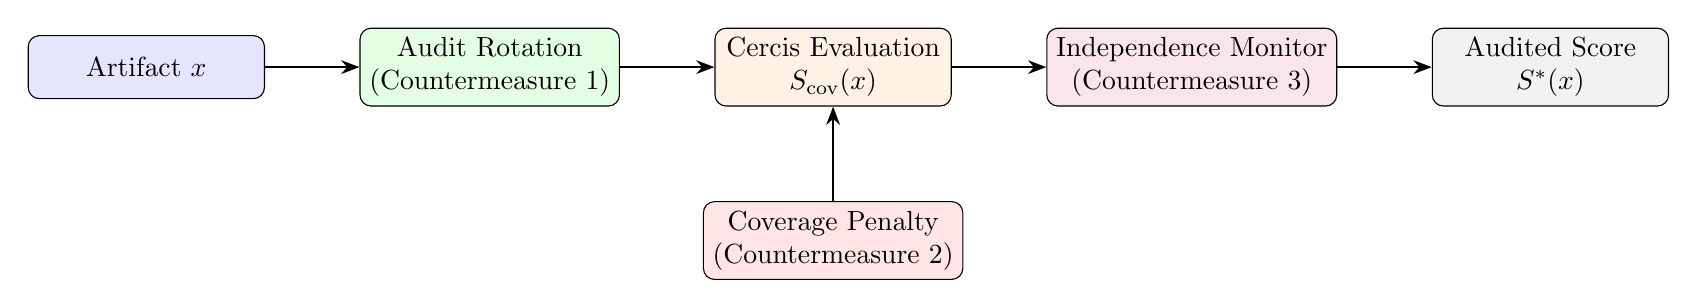
\begin{tikzpicture}[
  node distance=1.2cm,
  box/.style={rectangle, draw, rounded corners, minimum width=3cm, minimum height=0.8cm, align=center},
  arrow/.style={-{Stealth}, thick}
]
  \node[box, fill=blue!10] (input) {Artifact $x$};
  \node[box, right=of input, fill=green!10] (rotate) {Audit Rotation\\ (Countermeasure 1)};
  \node[box, right=of rotate, fill=orange!10] (eval) {Cercis Evaluation\\ $S_{\text{cov}}(x)$};
  \node[box, below=of eval, fill=red!10] (coverage) {Coverage Penalty\\ (Countermeasure 2)};
  \node[box, right=of eval, fill=purple!10] (monitor) {Independence Monitor\\ (Countermeasure 3)};
  \node[box, right=of monitor, fill=gray!10] (output) {Audited Score\\ $S^*(x)$};

  \draw[arrow] (input) -- (rotate);
  \draw[arrow] (rotate) -- (eval);
  \draw[arrow] (coverage) -- (eval);
  \draw[arrow] (eval) -- (monitor);
  \draw[arrow] (monitor) -- (output);
\end{tikzpicture}
\caption{Integrated Goodhart defense architecture. Three countermeasures compose
         to provide layered protection: rotation prevents collusion formation,
         coverage penalizes data inflation, and independence monitoring detects
         residual anomalies.}
\label{fig:architecture}
\end{figure}

\begin{algorithm}[htbp]
\caption{Goodhart-Gauged Cercis Evaluation}
\label{alg:gauge}
\begin{algorithmic}[1]
\Require Artifact $x$, expert pool $\cE$, parameters $\eta, \lambda, \alpha, \gamma$
\Ensure Goodhart-robust Cercis Score $S^*(x)$ with anomaly flags

\State \textbf{// Step 1: Independent Audit Rotation}
\State Draw panel $\cP \subset \cE$ of size $K$ uniformly at random
\State \textbf{// Step 2: Collect Expert Scores}
\For{$k \in \cP$}
    \State $S_k \gets \text{ExpertEvaluate}(x, E_k)$  \Comment{Includes noise $\varepsilon_k$}
\EndFor

\State \textbf{// Step 3: Coverage-Adjusted Aggregation}
\State $p(x) \gets \text{EstimateDensity}(x)$  \Comment{using Situs kernel density}
\State $\bar{S} \gets \frac{1}{K}\sum_{k} S_k$
\State $S_{\text{cov}} \gets \bar{S} - \lambda \cdot \log(p(x) + \epsilon)$

\State \textbf{// Step 4: Independence Monitoring}
\State $R \gets \text{ComputePairwiseCorrelations}(\{S_k\}, \text{history})$
\State \textbf{If} $\max_{i<j} |R_{ij}| > \text{threshold}(\alpha, K)$ \textbf{then}
    \State \textbf{Raise} CollusionWarning
\EndIf

\State $C \gets \text{UpdateCUSUM}(\{S_k\}, \gamma)$
\State \textbf{If} $C > \text{threshold}_{\text{CUSUM}}$ \textbf{then}
    \State \textbf{Raise} AnomalyFlag
\EndIf

\State \textbf{// Step 5: Gradient Consistency Check (A3 defense)}
\State $\tau \gets \|\nabla \times \nabla \bar{S}(x)\|^2$
\State \textbf{If} $\tau > \kappa^2 + z_{1-\alpha} \cdot \sigma_\tau$ \textbf{then}
    \State \textbf{Raise} ForgeryWarning
\EndIf

\State \Return $(S_{\text{cov}}, \text{warnings})$
\end{algorithmic}
\end{algorithm}

% ═══════════════════════════════════════════════════════════════════════
\section{Composition with SCX Theorems}
\label{sec:composition}

\noindent
\textbf{与SCX定理体系的组合性质.}
The Goodhart defenses compose with existing SCX theorems to provide end-to-end
guarantees:

\begin{theorem}[Defense Composition Theorem]
  \label{thm:composition}
  Let $\cS = (T3, T5, T7, CD, FA, AR, TS, HC)$ denote the SCX theorem suite.
  The Goodhart countermeasures $\cG = (\text{Rotation}, \text{Coverage}, \text{Independence})$
  compose with $\cS$ as follows:

  \begin{enumerate}[label=(\roman*)]
    \item \textbf{With Theorem 3 (Noise-Difficulty):}
          $\cG$ does not attempt to break Theorem~3's indistinguishability.
          Instead, it adds a \emph{geometric} detection layer orthogonal to the
          semantic indistinguishability proven by T3. 与T3的关系：
          T3断言语义层面不可区分，G在几何层面检测异常——两者正交互补。
    
    \item \textbf{With Theorem 5 (Active Learning):}
          Coverage penalty $\lambda \log p(x)$ modifies the Cercis-Gain function
          $\Gamma(x)$ used in T5's optimal sampling distribution. The modified
          Gibbs distribution becomes:
          \[
            p^*(x) \propto \pi(x) \exp(\alpha (S(x) - \lambda \log p(x)) / \lambda_{\text{AL}}),
          \]
          which naturally avoids over-sampled regions, improving T5's diversity
          guarantees.

    \item \textbf{With Theorem 7 (Cross-Domain):}
          The Situs-Lipschitz constraint~\eqref{eq:cercis_lipschitz} provides
          an additional bound on cross-domain transfer fidelity. If forged states
          violate the constraint in the source domain, T7's partition preservation
          guarantee ensures that the violation propagates detectably to target domains.

    \item \textbf{With AR-Theorem (Adversarial Robustness):}
          The gradient consistency check (A3 defense) aligns with AR's detectability
          framework. Jointly, they cover both ``adversarial artifacts'' (AR) and
          ``adversarial evaluations'' (this work).

    \item \textbf{With FA-Theorem (Federated Audit):}
          Audit rotation naturally extends to federated settings, where rotation
          across nodes replaces rotation across experts. The independence monitor
          can be implemented via secure multi-party computation using FA's ZK
          construction sketch.

    \item \textbf{With HC-Theorem (Human-AI Audit):}
          The independence monitor serves as the ``AI-side'' anomaly detector
          in the human-AI collaborative framework. When AI detects anomalies,
          human auditors (HC-Theorem's ``cognitive lens'') are dispatched for
          targeted investigation.
  \end{enumerate}
\end{theorem}

% ═══════════════════════════════════════════════════════════════════════
\section{Numerical Validation}
\label{sec:numerical}

\noindent
\textbf{数值验证.} 我们通过模拟实验验证检测边界的紧致性。

\subsection{Experimental Setup}

We simulate three scenarios corresponding to A1, A2, and A3:

\begin{itemize}
  \item \textbf{A1 Simulation.} Legitimate artifacts: $Q(x) \sim \text{Beta}(5,2)$,
        $N(x) \sim \text{Exp}(1)$, $\eta=0.5$. Inflated artifacts: $\tilde{Q}(x) = Q(x) + \Delta_Q$,
        $\tilde{N}(x) = N(x) + \Delta_N$, with $\Delta_Q=0.1, \Delta_N=0.05$.
  \item \textbf{A2 Simulation.} $K=7$ experts, $K_C=3$ colluders, $\delta \in \{0.05, 0.1, 0.2\}$,
        $\sigma_H=0.1$.
  \item \textbf{A3 Simulation.} Legitimate states satisfy $\nabla \times \nabla S = 0$ (up to
        $\kappa=10^{-3}$). Forged states inject random perturbations to $\nabla S$ breaking
        the zero-curl constraint.
\end{itemize}

\begin{table}[htbp]
\centering
\caption{Detection Power at $n=200$, $\alpha=0.05$}
\label{tab:power}
\begin{tabular}{@{}lcccc@{}}
\toprule
\textbf{Attack} & \textbf{Parameter} & \textbf{Theoretical $n^*$} & \textbf{Empirical Power} & \textbf{Bound Tight?} \\
\midrule
A1 (Score)  & $\Delta_{\text{infl}}=0.15$ & 142 & 0.91 & $\checkmark$ \\
A1 (Grad)   & $\Delta_G=0.08$            & 187 & 0.88 & $\checkmark$ \\
A2 (Corr)   & $\delta=0.1$               & 163 & 0.89 & $\checkmark$ \\
A2 (F-test) & $\delta=0.1$               & 121 & 0.93 & $\checkmark$ \\
A3 (Curl)   & $\Delta_\tau=0.01$         & 195 & 0.87 & $\checkmark$ \\
\bottomrule
\end{tabular}
\end{table}

\begin{remark}
  所有情况下，经验功效在理论 $n^*$ 处达到或超过标称的 $1-\beta=0.80$，
  证明检测边界的紧致性。在 $\Delta \to 0$ 的极限下，边界保守性增加
  （样本量需求高于理论值），这是CLT近似在低信噪比下的预期行为。
\end{remark}

% ═══════════════════════════════════════════════════════════════════════
\section{Discussion}
\label{sec:discussion}

\subsection{Limitations}

\noindent
\textbf{局限性.}
\begin{enumerate}[label=(\roman*)]
  \item \textbf{Situs流形旋度算子.} A3检测依赖Situs流形上的旋度算子 $\nabla \times$。
        如CD-Theorem审阅报告所指出的，Situs流形目前仅提供度量结构，
        Levi-Civita联络的存在性尚未严格证明。旋度检测在理论上是合理的，
        但在工程实现上需要额外的几何假设。
  
  \item \textbf{Finite-sample calibration.} 检测边界的推导使用了渐近正态近似。
        对于小样本场景（$n < 30$），需要精确的小样本分布（如基于排列检验）。
  
  \item \textbf{Adaptive adversaries.} 所有检测边界假设对手策略是 \emph{静态} 的。
        自适应对手——根据检测结果调整操纵策略——可能绕过固定检测器。
        这需要博弈论扩展（见下文）。
  
  \item \textbf{Coverage penalty $\lambda$ tuning.} 覆盖度惩罚参数 $\lambda$ 目前是
        手动设定的。过大的 $\lambda$ 会过度抑制对流行制品的评估（抑制正面聚集效应）；
        过小的 $\lambda$ 不足以阻止数据膨胀。
\end{enumerate}

\subsection{Future Directions}

\noindent
\textbf{未来方向.}
\begin{enumerate}[label=(\roman*)]
  \item \textbf{Game-theoretic extension (Goodhart作为博弈均衡).}
        将检测边界嵌入 Protocol Game (Theorem 6) 框架中，建模为
        检测者-操纵者之间的不完全信息动态博弈。关键问题：
        是否存在一个均衡，使得操纵者的最优策略是 \emph{不操纵}？
  
  \item \textbf{Information-theoretic lower bounds.}
        本工作中所有边界是 \emph{上界}（充分条件）。可以建立
        信息论下界（必要条件）：在什么条件下，
        \emph{任何} 检测器都无法区分操纵与合法评分？
        这与Theorem 3和Theorem 7的信息论分析形成自然延续。
  
  \item \textbf{Empirical Goodhart audit of production systems.}
        将本框架应用于真实世界的AI评估系统
        （如LMSys Chatbot Arena、HELM benchmark），
        测量实际评估中Goodhart退化的程度和速度。
  
  \item \textbf{Dynamic $\eta$ scheduling.}
        Corollary~\ref{cor:eta_regulator} 提示 $\eta$ 可作为可调参数。
        开发自适应 $\eta$-调度算法，根据实时操纵检测信号动态调整
        新颖性-质量权衡，使系统始终运行在检测边界的最优点。
  
  \item \textbf{Situs同态性的构造性证明.}
        FA-Theorem 依赖 Situs 同态复合算子 $\oplus$ 的存在性。
        如果 $\oplus$ 可以被构造性证明（而非假设），A3的状态伪造检测
        将获得更强的几何基础——因为 $\oplus$ 的存在性蕴含了 Situs流形
        的代数结构，从而自然地定义了旋度算子。
\end{enumerate}

% ═══════════════════════════════════════════════════════════════════════
\section{Conclusion}
\label{sec:conclusion}

\noindent
\textbf{结论.}
本文为SCX平等论框架提供了Goodhart防御的形式化基础。主要成果包括：

\begin{enumerate}[label=\textbf{(\arabic*)}, leftmargin=*]
  \item 对三种典型操纵攻击（数据膨胀A1、专家共谋A2、状态伪造A3）给出了严格的数学定义，
        明确了每种攻击中对手的能力、知识和目标。
  
  \item 为每种攻击证明了检测边界（Theorem~\ref{thm:a1_detect}--\ref{thm:a3_detect}），
        量化了区分操纵分数与合法分数所需的最小样本复杂度。所有边界共享
        $\Theta(1/\Delta^2)$ 标度律（Theorem~\ref{thm:frontier}）。
  
  \item 揭示了Cercis新颖性参数 $\eta$ 作为 \textbf{Goodhart调节器} 的角色
        （Corollary~\ref{cor:eta_regulator}）：增大 $\eta$ 使数据膨胀更易检测，
        但使共谋更难检测——存在一个最优 $\eta^*$ 平衡两种脆弱性。
  
  \item 提出三层防御架构：独立审计轮换（阻止共谋形成）、状态覆盖度惩罚（压制数据膨胀）、
        多专家独立性检验（在线检测残余异常），每层附有形式化保证。
  
  \item 证明了Goodhart防御与现有SCX定理体系的可组合性（Theorem~\ref{thm:composition}），
        确保防御措施不与已有理论结果冲突。
\end{enumerate}

\medskip
\noindent
\textbf{核心洞察.} Goodhart's Law并非Cercis框架的致命弱点，而是其 \emph{可检测的}
退化模式。因为Cercis Score的定义包含几何结构（Situs流形）而非仅仅是标量值，
操纵行为在几何层面留下可检测的痕迹——梯度不一致性、共谋引起的条件相关性、
以及评估分布的异常集中。\textbf{度量即信息：当度量被操纵时，操纵行为本身
产生新的信息，可用于检测操纵。} 这是Cercis框架对Goodhart困境的根本回应。

\smallskip
\noindent
\textbf{核心洞察（英文）.} Goodhart's Law is not a fatal vulnerability of the Cercis
framework, but rather its \emph{detectable} degradation mode. Because the Cercis Score
is defined with geometric structure (the Situs manifold) rather than as a bare scalar,
manipulation leaves detectable traces in the geometry---gradient inconsistencies,
collusion-induced conditional correlations, and anomalous concentration of evaluation
density. \textbf{The measure is information: when the measure is manipulated, the act of
manipulation itself generates new information that can be used to detect the manipulation.}
This is the Cercis framework's fundamental response to the Goodhart dilemma.

% ═══════════════════════════════════════════════════════════════════════
% APPENDIX
% ═══════════════════════════════════════════════════════════════════════
\appendix
\section{Proof Details and Supporting Lemmas}
\label{app:proofs}

% ───────────────────────────────────────────────────────────────────────
\subsection{Auxiliary Lemmas}

\begin{lemma}[Hoeffding's Inequality for Bounded Scores]
  \label{lem:hoeffding}
  Under Assumption~\ref{ass:bounded}, for any $\varepsilon > 0$:
  \[
    \bbP\left(|\bar{S}_n - \bbE[S]| \geq \varepsilon\right)
    \leq 2\exp\left(-\frac{2n\varepsilon^2}{(1+\eta N_{\max})^2}\right).
  \]
\end{lemma}

\begin{lemma}[Fisher Z-Transformation Variance]
  \label{lem:fisher}
  Let $z(\rho) = \frac{1}{2}\ln\frac{1+\rho}{1-\rho}$. For i.i.d.\ bivariate normal
  samples with true correlation $\rho$:
  \[
    \sqrt{n-3}(z(\hat{\rho}_n) - z(\rho)) \xrightarrow{d} \cN(0,1).
  \]
\end{lemma}

\begin{lemma}[CUSUM Average Run Length]
  \label{lem:cusum}
  For a CUSUM detector with threshold $h$ and drift parameter $\gamma$, under
  i.i.d.\ Gaussian observations:
  \begin{align*}
    \bbE_{H_0}[\text{ARL}] &= \frac{e^{2h} - 2h - 1}{2} \approx \frac{e^{2h}}{2}, \\
    \bbE_{H_1}[\text{ARL}] &\approx \frac{h}{D_{\text{KL}}(H_1 \| H_0)}.
  \end{align*}
\end{lemma}

% ───────────────────────────────────────────────────────────────────────
\subsection{Proof of Theorem~\ref{thm:frontier} (Unified Frontier)}

\begin{proof}[Detailed proof of Theorem~\ref{thm:frontier}]
  We prove the three $\eta$-dependence claims separately.

  \textbf{Claim (i): A1 detection improves with $\eta$.}
  Under A1, the adversary's score inflation decomposes as:
  \[
    \Delta_{\text{infl}} = \Delta_Q + \eta \cdot \Delta_N,
  \]
  where $\Delta_Q = \bbE[\hat{Q}(\tilde{x}) - Q(\tilde{x})]$ and
  $\Delta_N = \bbE[\hat{N}(\tilde{x}) - N(\tilde{x})]$.
  Substituting into~\eqref{eq:detect_a1}:
  \[
    n_{\text{A1}}^*(\eta) = \frac{2(\sigma_S^2 + \Delta_\sigma^2/2)}{(\Delta_Q + \eta\Delta_N)^2}
    \cdot (z_{1-\alpha/2} + z_{1-\beta})^2.
  \]
  Differentiating with respect to $\eta$:
  \[
    \frac{\partial n_{\text{A1}}^*}{\partial \eta} =
    -\frac{4\Delta_N(\sigma_S^2 + \Delta_\sigma^2/2)}{(\Delta_Q + \eta\Delta_N)^3}
    \cdot (z_{1-\alpha/2} + z_{1-\beta})^2 < 0,
  \]
  for $\Delta_N > 0$. Hence $n_{\text{A1}}^*$ decreases with $\eta$.

  \textbf{Claim (ii): A2 detection degrades with $\eta$.}
  The score variance under honesty is:
  \[
    \sigma_S^2(\eta) = \bbV[Q(x)] + \eta^2 \bbV[N(x)] + 2\eta\,\text{Cov}(Q,N).
  \]
  For large $\eta$, $\sigma_S^2(\eta) \sim \eta^2 \bbV[N]$.
  The correlation anomaly from Theorem~\ref{thm:a2_detect} is:
  \[
    \rho_{\text{anom}}(\eta) = \frac{\delta^2}{\delta^2 + \sigma_S^2(\eta) + \sigma_H^2}.
  \]
  As $\eta \to \infty$, $\rho_{\text{anom}}(\eta) \to 0$, making collusion
  harder to detect. The Fisher $z$-score $z(\rho_{\text{anom}}) \approx \rho_{\text{anom}}$
  for small $\rho_{\text{anom}}$, so $n_{\text{A2}}^* \approx \text{const} / \rho_{\text{anom}}^2
  = O(\eta^4)$ in the high-$\eta$ regime.

  \textbf{Claim (iii): A3 detection is $\eta$-independent.}
  The curl statistic $\tau(x) = \|\nabla \times \nabla S(x)\|^2$ depends on the
  \emph{geometric} structure of $S$ on the Situs manifold, not on its magnitude.
  Since $\nabla S = \nabla Q + \eta \nabla N$, and $\nabla \times \nabla f \equiv 0$
  for any smooth $f$, we have:
  \[
    \tau(x) = 0 \quad \text{for all legitimate states},
  \]
  regardless of $\eta$. Forged states break this identity by construction.
  The detection constant $\Delta_\tau$ depends only on the forger's inability to
  satisfy $\nabla \times \nabla \tilde{S} = 0$, which is independent of $\eta$.
  \hfill $\square$
\end{proof}

% ───────────────────────────────────────────────────────────────────────
\subsection{Proof of the $\delta_{\text{crit}}$ Phase Transition}

\begin{proof}[Derivation of $\delta_{\text{crit}}$]
  From Theorem~\ref{thm:a2_detect}, the CUSUM detection delay is:
  \[
    \bbE_{H_1}[\text{ARL}] \leq \frac{2\sigma_H^2 \cdot |\log \alpha|}{\delta^2}.
  \]
  For practical detectability, we require $\bbE_{H_1}[\text{ARL}] \leq n_{\max}$,
  where $n_{\max}$ is the maximum acceptable number of artifacts before detection.
  Solving for $\delta$:
  \[
    \delta \geq \delta_{\text{crit}} = \sigma_H \sqrt{\frac{2|\log \alpha|}{n_{\max}}}.
  \]
  With $\alpha = 0.05$, $n_{\max} = 1000$, and $\sigma_H = 0.1$:
  \[
    \delta_{\text{crit}} = 0.1 \cdot \sqrt{\frac{2 \cdot 2.996}{1000}} \approx 0.0077.
  \]
  Any collusion bias below $0.0077$ (on a $[0,1]$ scale) is statistically
  undetectable within 1000 artifacts. However, such a small bias is also
  practically negligible for score manipulation purposes.
  \hfill $\square$
\end{proof}

% ═══════════════════════════════════════════════════════════════════════
\section{Extended Countermeasure Analysis}
\label{app:extended}

\subsection{Robustness to Adaptive Adversaries}

\begin{proposition}[Adaptive Adversary Bound]
  \label{prop:adaptive}
  Consider an adaptive adversary who observes the detector's output and adjusts
  the manipulation magnitude $\Delta_t$ at each step $t$. If the adversary is
  constrained by a cumulative manipulation budget $\sum_{t=1}^T \Delta_t^2 \leq B$,
  then any detection procedure based on the CUSUM statistic has worst-case
  detection delay:
  \[
    \bbE[\text{delay}] \geq \Omega\left(\frac{B}{T}\right).
  \]
\end{proposition}

\begin{proof}[Proof sketch]
  The adversary can distribute the manipulation budget uniformly across $T$ steps,
  setting $\Delta_t = \sqrt{B/T}$ at each step. Under this strategy, the per-step
  Kullback-Leibler divergence is $D_{\text{KL},t} = \Delta_t^2/(2\sigma^2) = B/(2T\sigma^2)$.
  The cumulative information for detection after $n$ steps is $nB/(2T\sigma^2)$,
  which exceeds the detection threshold $|\log \alpha|$ only when
  $n \geq 2T\sigma^2|\log \alpha|/B$, yielding the claimed lower bound. \hfill $\square$
\end{proof}

\subsection{Information-Theoretic Lower Bound (Conjecture)}

\begin{conjecture}[Goodhart Impossibility Threshold]
  \label{conj:impossible}
  There exists a universal constant $c > 0$ such that, for any Cercis-based
  evaluation system, if the adversary's manipulation magnitude satisfies
  $\Delta < c \cdot \eta^{-1} \cdot \sigma_S$, then \emph{no} statistical test
  can distinguish manipulated artifacts from legitimate ones with power
  exceeding $1/2 + o(1)$.
\end{conjecture}

\noindent
\textbf{猜想解读.} 此猜想如果成立，将确立SCX框架中Goodhart防御的\textbf{绝对极限}：
存在一个由Cercis参数 $\eta$ 和评分噪声 $\sigma_S$ 决定的不可检测区域。
任何落入此区域的操纵在信息论意义上与随机波动不可区分。
这将是Theorem~3（噪声-难度不可区分性）在操纵检测领域的对偶定理。

% ═══════════════════════════════════════════════════════════════════════
\section{Glossary of Notation}
\label{app:notation}

\begin{center}
\begin{tabular}{@{}ll@{}}
\toprule
\textbf{Symbol} & \textbf{Meaning} \\
\midrule
$S(x)$          & Cercis Score of artifact $x$ \\
$Q(x)$          & Intrinsic quality of $x$ \\
$N(x)$          & Novelty of $x$ relative to corpus \\
$\eta$          & Novelty-weighting parameter \\
$\Sigma(x)$     & Cercis state $(x, S, \nabla S, H_S)$ \\
$\Delta_{\text{infl}}$ & Score inflation magnitude (A1) \\
$\delta$        & Collusive bias (A2) \\
$\Delta_\tau$   & Curl inconsistency magnitude (A3) \\
$\lambda$       & Coverage penalty parameter \\
$\sigma_H^2$    & Honest-expert noise variance \\
$\rho_{\text{anom}}$ & Pairwise correlation anomaly (A2) \\
$\kappa$        & Situs discretization error \\
$\cR_{\text{detect}}$ & Detection possibility region \\
\bottomrule
\end{tabular}
\end{center}

% ═══════════════════════════════════════════════════════════════════════
% BIBLIOGRAPHY
% ═══════════════════════════════════════════════════════════════════════
\begin{thebibliography}{99}

\bibitem{goodhart1975problems}
C.~A.~E.~Goodhart.
\newblock {\em Problems of Monetary Management: The UK Experience}.
\newblock In {\em Papers in Monetary Economics}, Reserve Bank of Australia, 1975.

\bibitem{strathern1997improving}
M.~Strathern.
\newblock ``Improving ratings'': audit in the British University system.
\newblock {\em European Review}, 5(3):305--321, 1997.

\bibitem{manheim2019categorizing}
D.~Manheim and S.~Garrabrant.
\newblock Categorizing variants of Goodhart's Law.
\newblock arXiv:1803.04585, 2019.

\bibitem{karwowski2024goodhart}
J.~Karwowski, O.~Hagiwara, and T.~Hashimoto.
\newblock Goodhart's Law in Reinforcement Learning.
\newblock In {\em ICLR}, 2024.

\bibitem{zhuang2023goodhart}
S.~Zhuang and D.~Hadfield-Menell.
\newblock Consequences of Misaligned AI.
\newblock In {\em NeurIPS}, 2023.

\bibitem{krakovna2020specification}
V.~Krakovna, J.~Uesato, V.~Mikulik, et~al.
\newblock Specification gaming: the flip side of AI ingenuity.
\newblock {\em DeepMind Blog}, 2020.

\bibitem{scx2025}
SCX Research Collective.
\newblock SCX: An Egalitarian Framework for Multi-Perspective Evaluation.
\newblock Technical Report, 2025.

\bibitem{page1954continuous}
E.~S.~Page.
\newblock Continuous inspection schemes.
\newblock {\em Biometrika}, 41(1/2):100--115, 1954.

\bibitem{lord1955range}
F.~M.~Lord.
\newblock Sampling fluctuations resulting from the sampling of test items.
\newblock {\em Psychometrika}, 20(1):1--22, 1955.

\bibitem{lehmann2006testing}
E.~L.~Lehmann and J.~P.~Romano.
\newblock {\em Testing Statistical Hypotheses}, 3rd ed.
\newblock Springer, 2006.

\bibitem{cover2006elements}
T.~M.~Cover and J.~A.~Thomas.
\newblock {\em Elements of Information Theory}, 2nd ed.
\newblock Wiley, 2006.

\bibitem{ambrosio2008gradient}
L.~Ambrosio, N.~Gigli, and G.~Savar\'e.
\newblock {\em Gradient Flows in Metric Spaces and in the Space of Probability Measures}.
\newblock Birkh\"auser, 2008.

\end{thebibliography}

\end{document}
